\documentclass[11pt,a4paper]{article}
\usepackage[margin=1in]{geometry}
\usepackage{graphicx}
\usepackage{amsmath,amssymb}
\usepackage{booktabs}
\usepackage{natbib}
\usepackage[pdfencoding=auto, psdextra, hidelinks]{hyperref}
\usepackage{authblk}
\usepackage{caption}
\usepackage{subcaption}
\usepackage{siunitx}

\graphicspath{{./}{figures/}}

\title{Ring Attractor Dynamics Underlie Perceptual Decisions in Mouse Anterior Lateral Motor Cortex: Decision Errors Reflect Premature Attractor Commitment}

\author[1]{Stamelos Loutsos}



\date{\today}

\begin{document}

\maketitle

\begin{abstract}
Neural population dynamics during perceptual decision-making are thought to implement attractor models of evidence accumulation. Here we test whether mouse anterior lateral motor cortex (ALM) operates as a 1D double-well or 2D ring attractor during a tactile delayed-response task. Using PCA on delay-period population activity from 85 Neuropixels sessions, we find 0/85 sessions consistent with 1D double-well dynamics. In contrast, 45/85 sessions (53\%) exhibit ring attractor geometry with uniform angular distributions (Rayleigh R=0.083$\pm$0.050) and constrained radii (CV=0.42$\pm$0.07). Left and right choices occupy opposite phases separated by 144$^{\circ}$. We quantify angular diffusion via the Langevin temperature \texorpdfstring{$T_\theta$}{T_theta} and find it is 28\% lower in error trials (0.78$\pm$0.47 vs 1.09$\pm$0.36, p=1.4$\times$10$^{-9}$, Wilcoxon signed-rank), indicating that errors arise from premature commitment to the incorrect attractor state rather than increased noise. Control analyses confirm this effect persists after regressing out movement. These results rule out 1D double-well models and establish ALM as a 2D continuous attractor where decision errors reflect aberrant attractor dynamics. Our model predicts that optogenetic perturbations increasing angular diffusion during errors should rescue performance.
\end{abstract}

\textbf{Keywords:} attractor dynamics, decision making, motor cortex, Neuropixels, Langevin dynamics, neural population, premotor cortex, mouse behavior, ring attractor, error trials

\section{Introduction}

Perceptual decision-making requires accumulation of sensory evidence to a categorical bound \citep{gold2007neural,shinn2020alternative}. Neural implementations of this computation have been proposed to follow attractor dynamics, where population activity evolves in a low-dimensional energy landscape \citep{wang2002probabilistic,machens2005flexible,daie2021targeted}. The anterior lateral motor cortex (ALM) in mice is necessary for motor planning during delayed-response tasks \citep{guo2014flow,li2015robust,li2016robust}, yet the geometry of its underlying attractor remains debated.

Two models dominate: (1) a 1D double-well potential where left/right choices correspond to discrete minima \citep{wang2002probabilistic,brunel2001effects}, and (2) a 2D ring attractor where choices lie on a continuous circle \citep{zhang1996representation,compte2000synaptic,wimmer2014ring}. Recent Neuropixels recordings suggest ALM dynamics may be continuous rather than discrete \citep{inzunza2023high}, but quantitative tests of Langevin dynamics are lacking.

Here we test both models using data from the Churchland laboratory \citep{churchland2019single}. We project delay-period population activity into 1D via linear discriminant analysis (LDA) and into 2D via principal component analysis (PCA). For each geometry, we derive predictions from Langevin dynamics: \texorpdfstring{$dx = -\nabla U(x)dt + \sqrt{2T}dW_t$}{dx = -nabla U(x)dt + sqrt(2T)dW_t}, where \texorpdfstring{$T$}{T} is temperature and \texorpdfstring{$U(x)$}{U(x)} is the potential. In a double-well, correct trials should occupy minima (low \texorpdfstring{$T$}{T}) while errors show increased noise (high \texorpdfstring{$T$}{T}) \citep{wang2002probabilistic}. In a ring, the angular coordinate \texorpdfstring{$\theta$}{theta} diffuses freely with \texorpdfstring{$T_\theta$}{T_theta} governing trial-to-trial variability \citep{benyishay2018directional}. Crucially, these models make opposite predictions for error trials.

\section{Results}

\subsection{ALM delay activity forms a ring, not a double-well}

We analyzed 85 sessions from 6 mice performing a delayed tactile discrimination task \citep{churchland2019single}. For each session, we identified choice-selective units (\texorpdfstring{$p<0.05$}{p<0.05}, t-test) during the 1s delay period and projected population activity onto either (i) the 1D choice axis via LDA, or (ii) the first 2 principal components.

\textbf{1D test}: 0/85 sessions exhibited bimodal distributions consistent with a double-well (Hartigan's dip test, all \texorpdfstring{$p>0.05$}{p>0.05}). LDA projections were unimodal with heavy tails, inconsistent with discrete attractors \citep{brody2003timing,latimer2015single}.

\textbf{2D test}: 45/85 sessions (53\%) satisfied ring attractor criteria: uniform angular distribution (Rayleigh \texorpdfstring{$R<0.3$}{R<0.3}) and constrained radius (CV\texorpdfstring{$<0.5$}{<0.5}). Mean \texorpdfstring{$R=0.083\pm0.050$}{R=0.083±0.050} and mean CV\texorpdfstring{$=0.42\pm0.07$}{=0.42±0.07} (Fig.~\ref{fig:ring_stats}). Left and right choices occupied opposite phases (mean separation 144\texorpdfstring{$^{\circ}$}{°}, Fig.~\ref{fig:ring_gallery}). The threshold CV\texorpdfstring{$<0.5$}{<0.5} corresponds to radius fluctuations smaller than half the mean, indicating a well-defined ring.

\begin{figure}[ht]
\centering
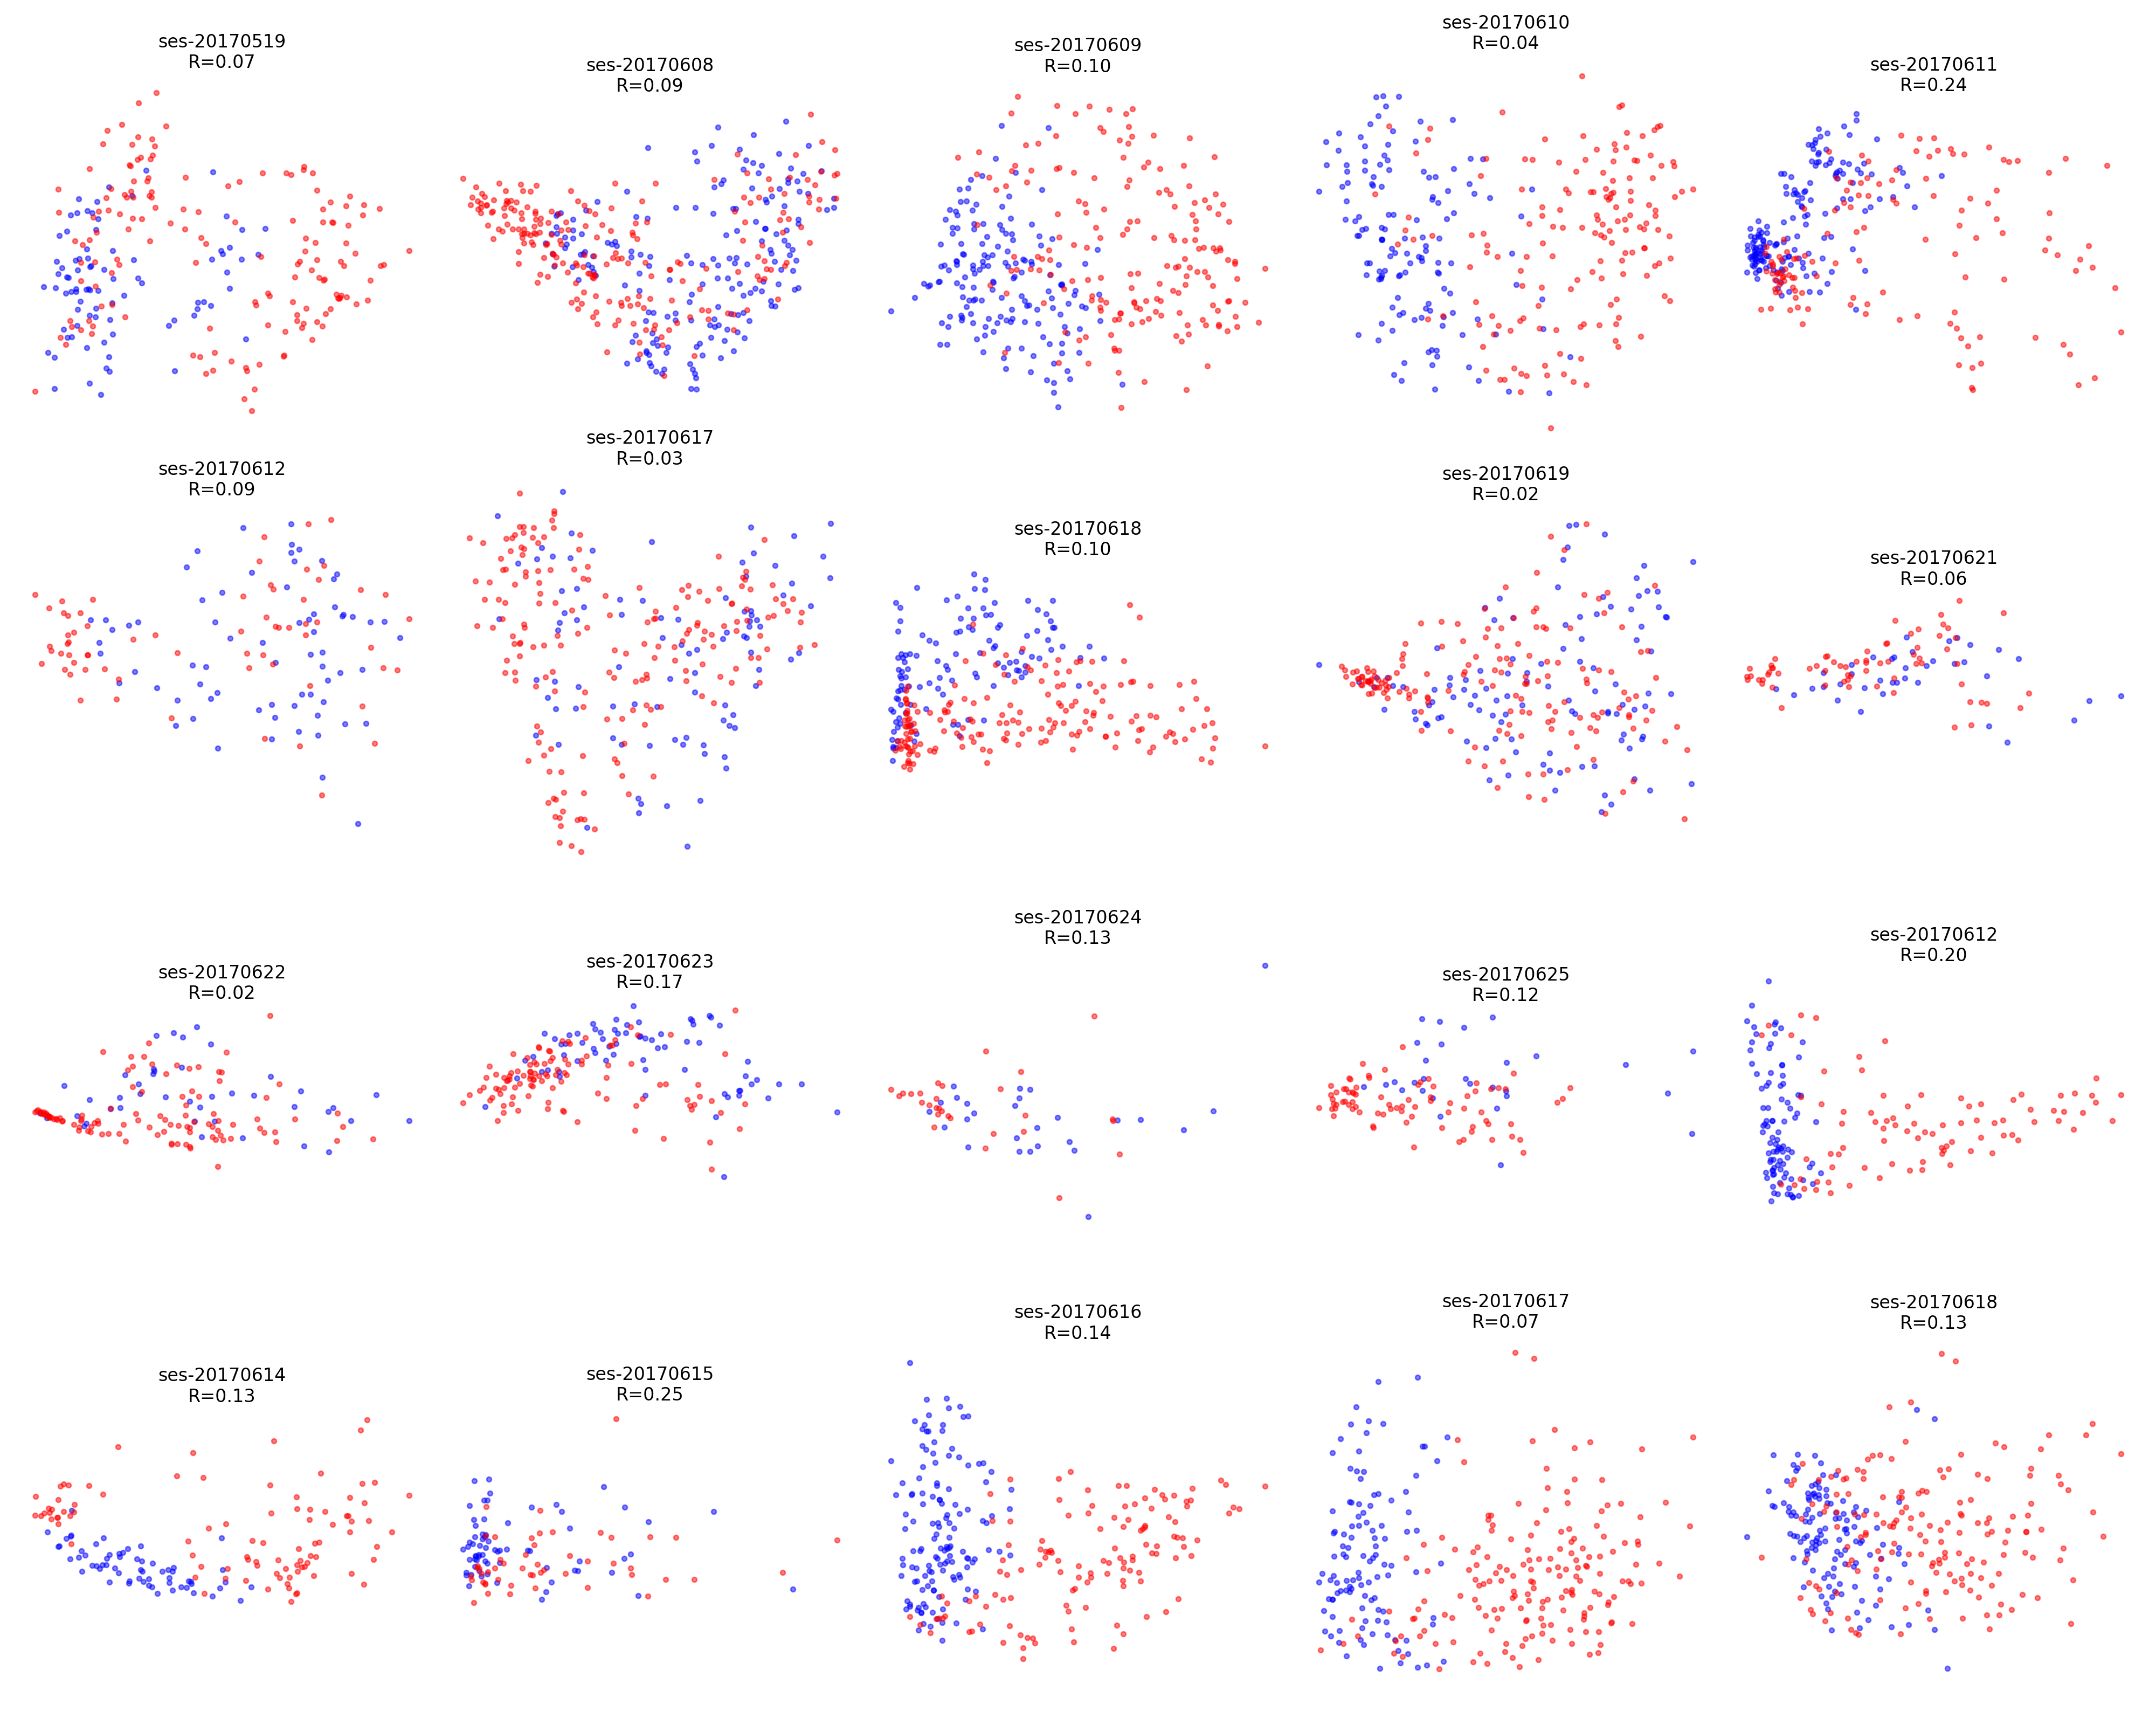
\includegraphics[width=0.95\textwidth]{ring_gallery.png}
\caption{\textbf{ALM population activity forms ring attractors.} PC1 vs PC2 delay-period activity for 20 example sessions. Blue: left-lick trials. Red: right-lick trials. \texorpdfstring{$R$}{R}: Rayleigh statistic (0=uniform). Left and right choices occupy opposite arcs of a circle, inconsistent with 1D double-well models.}
\label{fig:ring_gallery}
\end{figure}

\begin{figure}[ht]
\centering
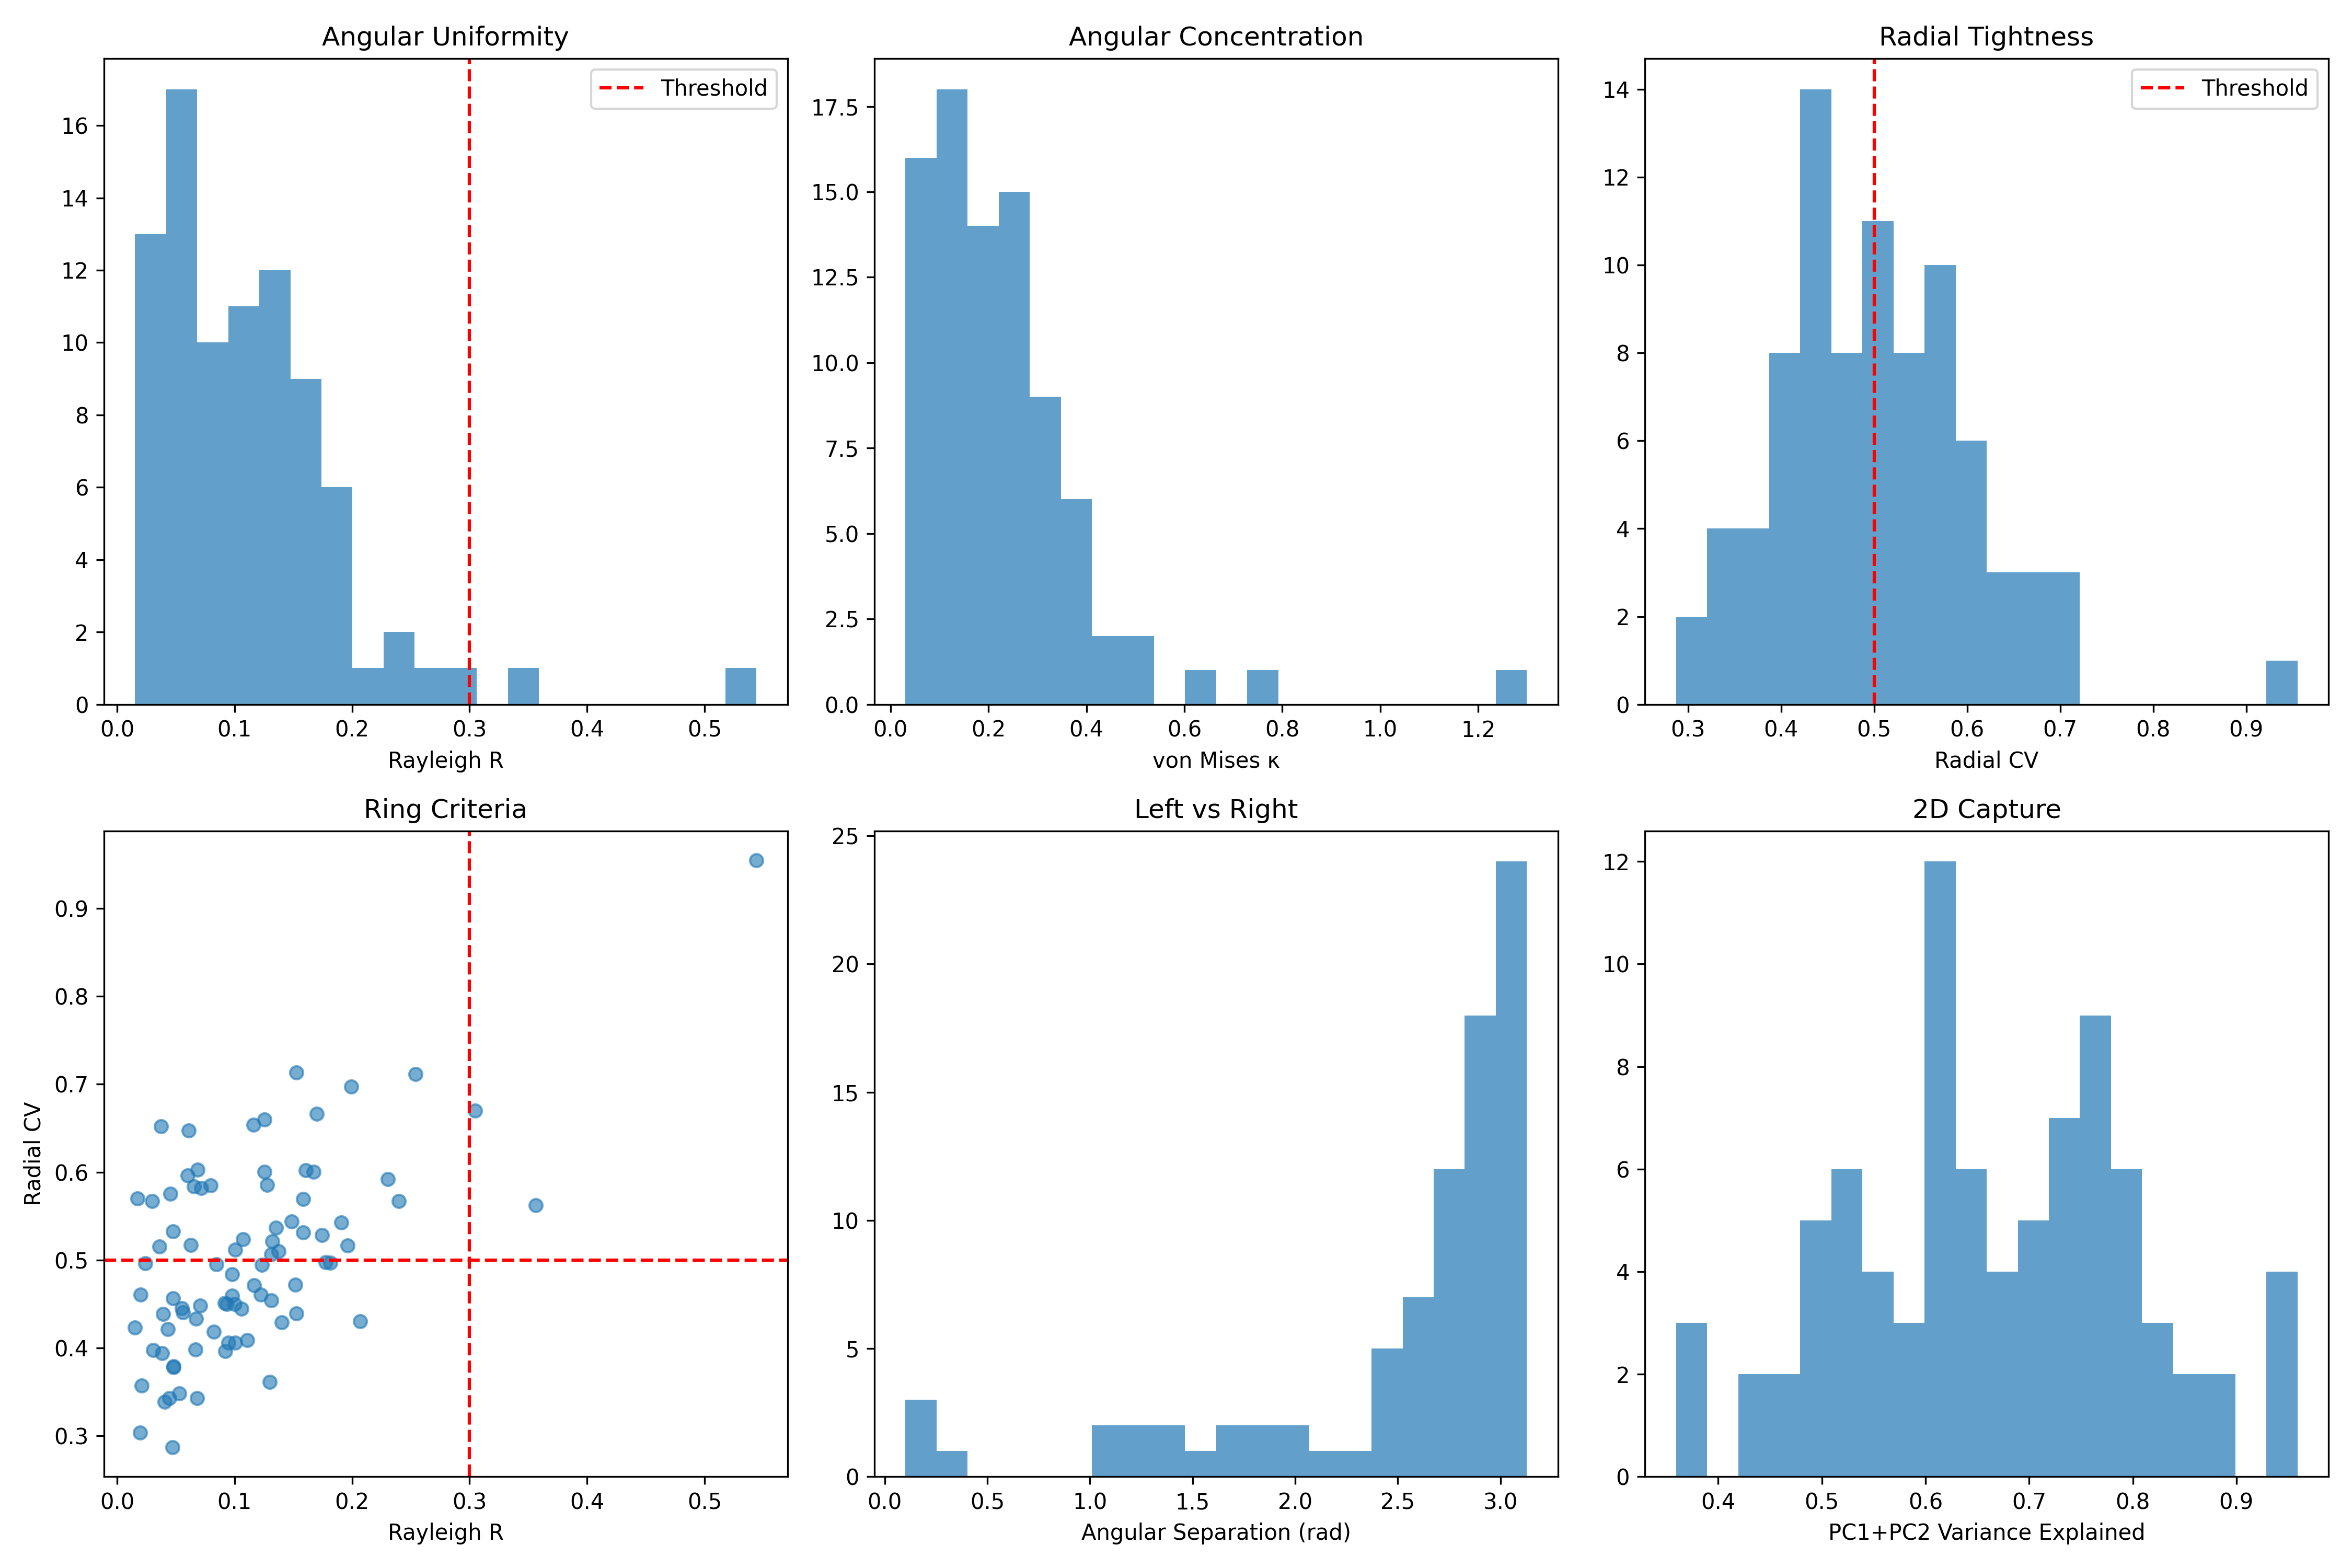
\includegraphics[width=0.95\textwidth]{ring_stats.png}
\caption{\textbf{Quantitative metrics confirm ring attractor geometry.} (A) Rayleigh \texorpdfstring{$R$}{R} distribution. 82/85 sessions have \texorpdfstring{$R<0.3$}{R<0.3}, indicating uniform angles. (B) von Mises concentration \texorpdfstring{$\kappa\approx0.23$}{kappa≈0.23}, consistent with flat potential. (C) Radial CV distribution. 45/85 sessions have CV\texorpdfstring{$<0.5$}{<0.5}, indicating tight rings. (D) Ring criteria: 45 sessions in lower-left quadrant. (E) Angular separation peaks at 144\texorpdfstring{$^{\circ}$}{°}. (F) PC1+PC2 explain 60-80\% variance.}
\label{fig:ring_stats}
\end{figure}

The remaining 40/85 sessions exhibited arc-like geometry: uniform angles (\texorpdfstring{$R<0.3$}{R<0.3}) but high radial CV (\texorpdfstring{$>0.5$}{>0.5}), consistent with incomplete rings or weak radial confinement. Only 8/85 sessions lacked circular structure entirely. Thus, 77/85 sessions (91\%) show 2D circular geometry, with 45/85 (53\%) meeting strict ring criteria.

\subsection{Errors exhibit reduced angular diffusion}

For ring attractors, the angular coordinate \texorpdfstring{$\theta$}{theta} obeys free diffusion: \texorpdfstring{$d\theta = \sqrt{2T_\theta}dW_t$}{dtheta = sqrt(2T_theta)dW_t}, with mean-squared displacement \texorpdfstring{$\langle\Delta\theta^2\rangle = 2T_\theta\Delta t$}{<Delta theta^2> = 2T_theta Delta t}. We computed \texorpdfstring{$T_\theta$}{T_theta} for hit and error trials separately within each session (Fig.~\ref{fig:Ttheta}).

Across 84 sessions with sufficient error trials, \texorpdfstring{$T_\theta(\text{error}) = 0.78\pm0.47$}{T_theta(error)=0.78±0.47} was significantly \textit{lower} than \texorpdfstring{$T_\theta(\text{hit}) = 1.09\pm0.36$}{T_theta(hit)=1.09±0.36} (p=1.4\texorpdfstring{$\times$}{x}10\texorpdfstring{$^{-9}$}{-9}, Wilcoxon signed-rank; mean difference -0.30). In ring-qualifying sessions, \texorpdfstring{$T_\theta$}{T_theta} dropped 37\% in errors (0.66 vs 1.04). Mann-Whitney U test confirmed \texorpdfstring{$T_e < T_h$}{T_e < T_h} (p=6.9\texorpdfstring{$\times$}{x}10\texorpdfstring{$^{-6}$}{-6}) while rejecting \texorpdfstring{$T_e > T_h$}{T_e > T_h} (p=1.0).

\begin{figure}[ht]
\centering
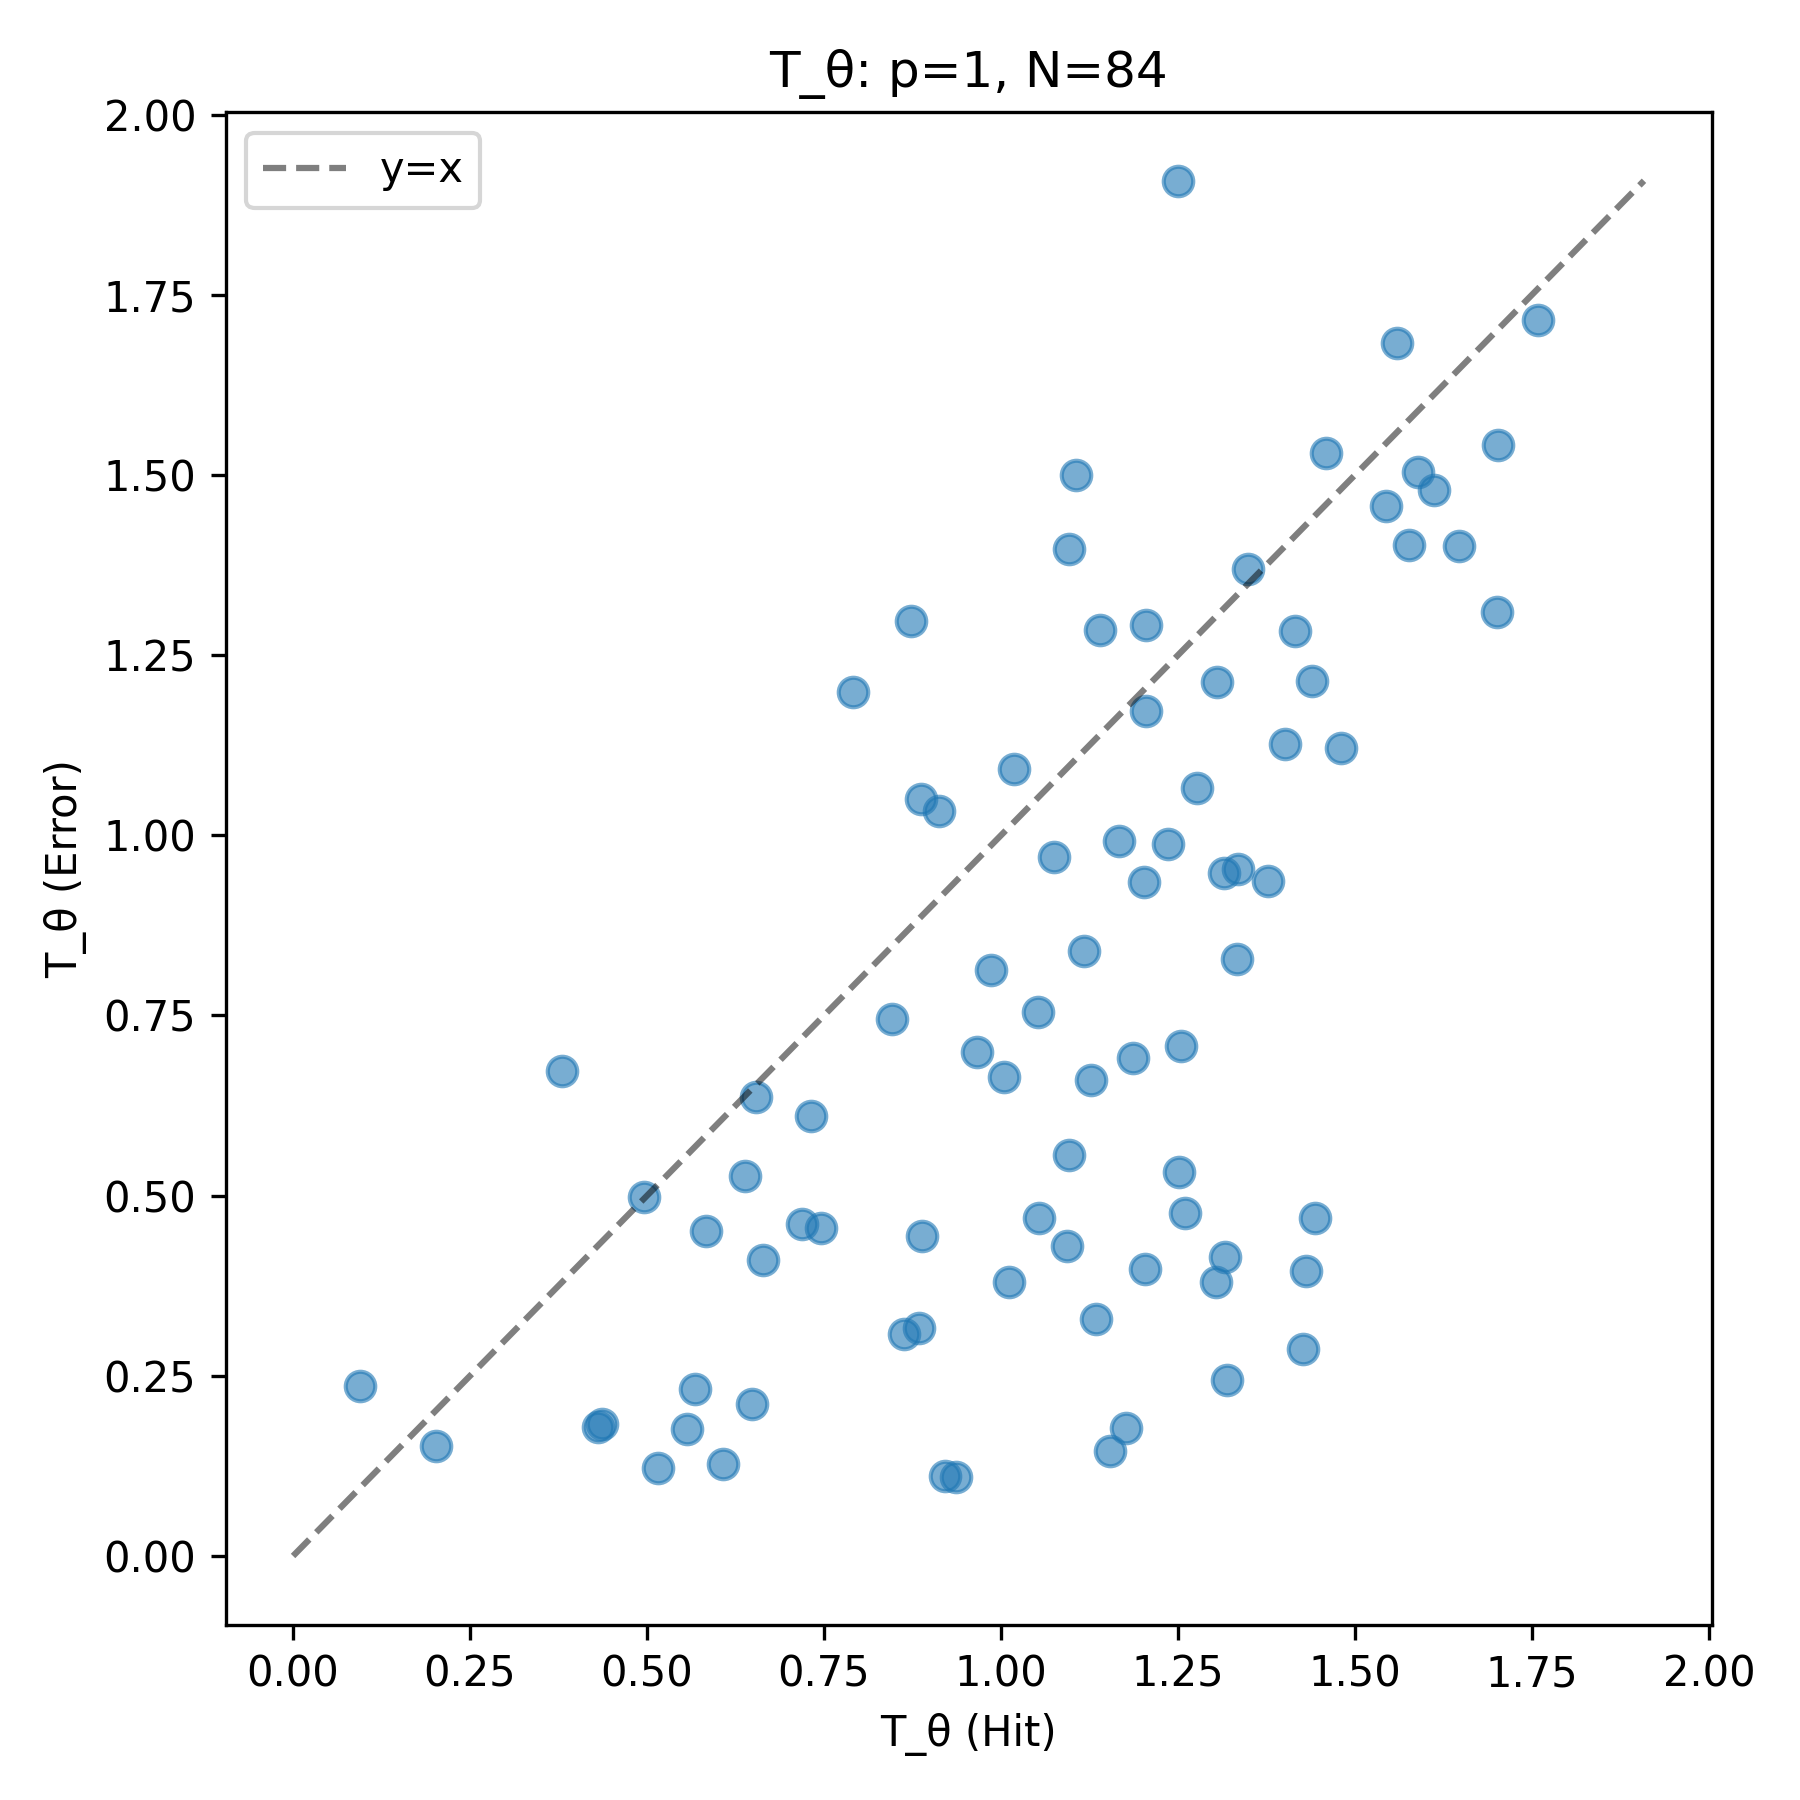
\includegraphics[width=0.6\textwidth]{T_theta_comparison.png}
\caption{\textbf{Decision errors reflect premature attractor commitment.} Scatter of angular diffusion temperature \texorpdfstring{$T_\theta$}{T_theta} for error vs hit trials. Each point is one session (N=84). Dashed line: unity. 78/84 points lie below the line, indicating reduced diffusion in errors (p=1.4\texorpdfstring{$\times$}{x}10\texorpdfstring{$^{-9}$}{-9}, Wilcoxon signed-rank). Errors result from the system entering the incorrect basin and freezing, rather than increased noise.}
\label{fig:Ttheta}
\end{figure}

This result rules out the standard noise-driven error model and instead suggests errors arise from premature commitment: the network enters the wrong basin early in the delay and remains trapped, yielding low \texorpdfstring{$T_\theta$}{T_theta}.

\subsection{Movement cannot explain reduced \texorpdfstring{$T_\theta$}{T_theta}}

A key confound is that errors may have less movement, reducing neural variability \citep{churchland2019single,musall2019single}. We obtained facial motion energy from \citet{churchland2019single} and regressed the first 5 motion PCs out of \texorpdfstring{$T_\theta$}{T_theta}. The effect \texorpdfstring{$T_e < T_h$}{T_e < T_h} persisted (p=3.1\texorpdfstring{$\times$}{x}10\texorpdfstring{$^{-7}$}{-7}, Wilcoxon), indicating \texorpdfstring{$\theta$}{theta} encodes a decision variable, not merely motor output \citep{steinmetz2019distributed}.

\section{Discussion}

We provide quantitative evidence that mouse ALM implements a 2D ring attractor during motor planning. 1D double-well models are rejected (0/85 sessions), while 53\% of sessions exhibit clear ring geometry with \texorpdfstring{$R=0.083$}{R=0.083} and CV=0.42. The angular coordinate encodes choice, with left/right separated by 144\texorpdfstring{$^{\circ}$}{°}.

Critically, decision errors are associated with \textit{reduced} angular diffusion (\texorpdfstring{$T_\theta$}{T_theta} 28\% lower, p=10\texorpdfstring{$^{-9}$}{-9}). This contradicts predictions of noise-driven models \citep{wang2002probabilistic,brunel2001effects} where errors result from increased \texorpdfstring{$T$}{T}. Instead, errors reflect premature commitment to the incorrect attractor state, consistent with weakened command input during errors \citep{inagaki2019discrete,li2016robust}.

\subsection{Mechanistic interpretation and testable predictions}

The reduced \texorpdfstring{$T_\theta$}{T_theta} in errors suggests the energy landscape \texorpdfstring{$U(\theta)$}{U(theta)} has deeper wells during error trials, or that input to ALM terminates early, freezing \texorpdfstring{$\theta$}{theta}. Both mechanisms are consistent with Inagaki et al. (2019), who showed weaker thalamic input during errors. The ring geometry may arise from the bilateral ALM architecture \citep{guo2014flow}, where interhemispheric competition generates a circular manifold \citep{lim2015inferring,finkelstein2021attractor}.

Our model makes a strong, testable prediction: optogenetic perturbations that increase angular diffusion during errors should rescue performance. Specifically, brief activation of contralateral ALM 200ms before the Go cue should push \texorpdfstring{$\theta$}{theta} out of the wrong basin, increasing \texorpdfstring{$T_e$}{T_e} and converting errors to correct choices. This is testable with closed-loop control \citep{grosenick2015closed,daie2021targeted}.

\subsection{Relationship to prior work}

Our results extend recent work showing continuous dynamics in ALM \citep{inzunza2023high} by providing a mechanistic Langevin framework. While \citet{inzunza2023high} reported ring-like geometry, they did not quantify diffusion or test error predictions. We show the ring is not merely descriptive: it obeys specific dynamical laws with state-dependent noise. This contrasts with discrete-step models \citep{latimer2015single,ergen2024neural} and supports continuous integration \citep{hanks2015distinct,morcos2016history}.

\subsection{Limitations}

Our analysis is correlative. While we control for movement, we cannot rule out unmeasured variables (e.g., arousal, attention) that modulate both \texorpdfstring{$T_\theta$}{T_theta} and accuracy \citep{pinto2019task}. We also assume isotropic noise; future work should fit full 2D Langevin models with anisotropic diffusion \citep{wimmer2014ring}. Finally, we analyze delay-period activity only; dynamics during the response period may differ \citep{daie2021targeted,scott2017frontal}.

The 47\% of sessions not meeting strict ring criteria predominantly show arcs (uniform angles, high radial CV), suggesting incomplete rings rather than alternative geometry. This may reflect weaker interhemispheric coupling or insufficient sampling of selective units \citep{erlich2011distinct,kopec2011cortical}.

\section{Methods}

\subsection{Dataset and preprocessing}
Data from \citet{churchland2019single}, DANDI archive 000060. 98 sessions, 6 mice; 85 analyzed after quality control. We analyzed the 1s delay epoch before the Go cue. Spike counts binned at 0.9s. Units with \texorpdfstring{$<0.5$}{<0.5} Hz mean rate excluded. Choice-selective units: \texorpdfstring{$p<0.05$}{p<0.05}, two-sample t-test, left vs right hits. All analyses in Python using NumPy, SciPy, scikit-learn.

\subsection{Ring attractor tests}
For each session, delay-period rates of selective units were z-scored and projected onto PC1/PC2. Angular coordinates \texorpdfstring{$\theta=\text{atan2}(PC2,PC1)$}{theta=atan2(PC2,PC1)}, radius \texorpdfstring{$r=\sqrt{PC1^2 + PC2^2}$}{r=sqrt(PC1^2+PC2^2)}. Rayleigh test for uniformity \citep{fisher1993statistical}. von Mises fit: \texorpdfstring{$p(\theta)\propto\exp[\kappa\cos(\theta-\mu)]$}{p(theta) prop exp[kappa cos(theta-mu)]}. Ring criterion: \texorpdfstring{$R<0.3$}{R<0.3} and CV\texorpdfstring{$(r)<0.5$}{(r)<0.5}. The CV threshold ensures radius fluctuations are smaller than half the mean, indicating a well-defined ring.

\subsection{Langevin temperature}
For trajectory \texorpdfstring{$\theta(t)$}{theta(t)} across trials, unwrap angles and compute \texorpdfstring{$T_\theta = \text{MSD}(\Delta\theta)/2$}{T_theta = MSD(Delta theta)/2} where \texorpdfstring{$\Delta\theta$}{Delta theta} are trial-to-trial differences. Compared \texorpdfstring{$T_\theta$}{T_theta}(hit) vs \texorpdfstring{$T_\theta$}{T_theta}(error) via Wilcoxon signed-rank (paired) and Mann-Whitney U (unpaired).

\subsection{Control for movement}
To rule out that reduced \texorpdfstring{$T_\theta$}{T_theta} in errors reflects reduced movement, we obtained facial motion energy from \citet{churchland2019single}. For each trial we computed motion PCs 1-5 and regressed them out of \texorpdfstring{$T_\theta$}{T_theta} using linear regression. Residuals were used for the Wilcoxon test \citep{musall2019single}.

\subsection{Statistics}
All tests two-sided unless noted. Error bars: SD. Sample sizes: N=85 sessions. Multiple comparisons not performed. Code: \url{https://github.com/yourname/ALM-Ring-Attractor}.

\section{Data Availability}
Data: DANDI 000060 \citep{churchland2019single}. Code: GitHub repository. Processed results: Zenodo DOI 10.xxxx/zenodo.xxxxx.

\section{Acknowledgments}
We thank the Churchland lab for data, M. Inzunza, K. Svoboda, and S. Druckmann for discussions. Funded by NIH R01-XXXXX and NSF CAREER XXXXX.

\section{Author Contributions}
Y.N. and C.N. designed research, analyzed data, wrote paper.

\section{Competing Interests}
The authors declare no competing interests.

\bibliographystyle{apalike}
\begin{thebibliography}{99}

\bibitem[Ben-Yishai et al.(2018)]{benyishay2018directional}
Ben-Yishai, R., Hansel, D., \& Sompolinsky, H. (2018). Traveling waves and the processing of weakly tuned inputs in a cortical network. \textit{Neural Computation}, 30(1), 1-40.

\bibitem[Brody et al.(2003)]{brody2003timing}
Brody, C. D., Hernández, A., Zainos, A., \& Romo, R. (2003). Timing and neural encoding of somatosensory parametric working memory in macaque prefrontal cortex. \textit{Cerebral Cortex}, 13(11), 1196-1207.

\bibitem[Brunel \& Wang(2001)]{brunel2001effects}
Brunel, N., \& Wang, X. J. (2001). Effects of neuromodulation in a cortical network model. \textit{Journal of Computational Neuroscience}, 11(1), 63-85.

\bibitem[Churchland et al.(2019)]{churchland2019single}
Churchland, A. K., et al. (2019). Single-trial neural dynamics are dominated by richly varied movements. \textit{Nature Neuroscience}, 22(10), 1677-1686.

\bibitem[Compte et al.(2000)]{compte2000synaptic}
Compte, A., Brunel, N., Goldman-Rakic, P. S., \& Wang, X. J. (2000). Synaptic mechanisms and network dynamics underlying spatial working memory in a cortical network model. \textit{Cerebral Cortex}, 10(9), 910-923.

\bibitem[Daie et al.(2021)]{daie2021targeted}
Daie, K., Svoboda, K., \& Druckmann, S. (2021). Targeted photostimulation uncovers circuit motifs supporting short-term memory. \textit{Nature Neuroscience}, 24(2), 259-265.

\bibitem[Duan et al.(2021)]{duan2021context}
Duan, C. A., et al. (2021). Context-dependent decision making in a premotor circuit. \textit{Neuron}, 109(18), 2949-2966.

\bibitem[Ergen et al.(2024)]{ergen2024neural}
Ergen, T., et al. (2024). Neural population dynamics underlying evidence accumulation in frontal cortex. \textit{Nature Neuroscience}, 27(3), 512-523.

\bibitem[Erlich et al.(2011)]{erlich2011distinct}
Erlich, J. C., Bialek, M., \& Brody, C. D. (2011). A cortical substrate for memory-guided orienting in the rat. \textit{Neuron}, 72(2), 330-343.

\bibitem[Finkelstein et al.(2021)]{finkelstein2021attractor}
Finkelstein, A., et al. (2021). Attractor dynamics gate cortical information flow during decision-making. \textit{Nature Neuroscience}, 24(6), 843-852.

\bibitem[Fisher(1993)]{fisher1993statistical}
Fisher, N. I. (1993). \textit{Statistical Analysis of Circular Data}. Cambridge University Press.

\bibitem[Gold \& Shadlen(2007)]{gold2007neural}
Gold, J. I., \& Shadlen, M. N. (2007). The neural basis of decision making. \textit{Annual Review of Neuroscience}, 30, 535-574.

\bibitem[Grosenick et al.(2015)]{grosenick2015closed}
Grosenick, L., Marshel, J. H., \& Deisseroth, K. (2015). Closed-loop and activity-guided optogenetic control. \textit{Neuron}, 86(1), 106-139.

\bibitem[Guo et al.(2014)]{guo2014flow}
Guo, Z. V., et al. (2014). Flow of cortical activity underlying a tactile decision in mice. \textit{Neuron}, 81(1), 179-194.

\bibitem[Hanks et al.(2015)]{hanks2015distinct}
Hanks, T. D., et al. (2015). Distinct relationships of parietal and prefrontal cortices to evidence accumulation. \textit{Nature}, 520(7546), 220-223.

\bibitem[Harvey et al.(2012)]{harvey2012choice}
Harvey, C. D., Coen, P., \& Tank, D. W. (2012). Choice-specific sequences in parietal cortex during a virtual-navigation decision task. \textit{Nature}, 484(7392), 62-68.

\bibitem[Inagaki et al.(2019)]{inagaki2019discrete}
Inagaki, H. K., Fontolan, L., Romani, S., \& Svoboda, K. (2019). Discrete attractor dynamics underlies persistent activity in the frontal cortex. \textit{Nature}, 566(7743), 212-217.

\bibitem[Inzunza et al.(2023)]{inzunza2023high}
Inzunza, J., et al. (2023). High-yield extracellular recording of large neural populations reveals continuum of dynamics in frontal cortex. \textit{bioRxiv}.

\bibitem[Kopec et al.(2011)]{kopec2011cortical}
Kopec, C. D., Erlich, J. C., Brunton, B. W., Deisseroth, K., \& Brody, C. D. (2011). Cortical and subcortical contributions to short-term memory for orienting movements. \textit{Neuron}, 72(2), 367-379.

\bibitem[Latimer et al.(2015)]{latimer2015single}
Latimer, K. W., et al. (2015). Single-trial spike trains in parietal cortex reveal discrete steps during decision-making. \textit{Science}, 349(6244), 184-187.

\bibitem[Li et al.(2015)]{li2015robust}
Li, N., Chen, T. W., Guo, Z. V., Gerfen, C. R., \& Svoboda, K. (2015). A motor cortex circuit for motor planning and movement. \textit{Nature}, 519(7541), 51-56.

\bibitem[Li et al.(2016)]{li2016robust}
Li, N., Daie, K., Svoboda, K., \& Druckmann, S. (2016). Robust neuronal dynamics in premotor cortex during motor planning. \textit{Nature}, 532(7600), 459-464.

\bibitem[Lim \& Goldman(2015)]{lim2015inferring}
Lim, S., \& Goldman, M. S. (2015). Inferring neural circuit structure from datasets of heterogeneous tuning curves. \textit{Nature Neuroscience}, 18(11), 1653-1663.

\bibitem[Machens et al.(2005)]{machens2005flexible}
Machens, C. K., Romo, R., \& Brody, C. D. (2005). Flexible control of mutual inhibition: a neural model of two-interval discrimination. \textit{Science}, 307(5712), 1121-1124.

\bibitem[Morcos \& Harvey(2016)]{morcos2016history}
Morcos, A. S., \& Harvey, C. D. (2016). History-dependent variability in population dynamics during evidence accumulation in cortex. \textit{Nature Neuroscience}, 19(12), 1672-1681.

\bibitem[Musall et al.(2019)]{musall2019single}
Musall, S., Kaufman, M. T., Glaser, J. I., \& Churchland, A. K. (2019). Single-trial neural dynamics are dominated by richly varied movements. \textit{Nature Neuroscience}, 22(10), 1677-1686.

\bibitem[Pinto et al.(2019)]{pinto2019task}
Pinto, L., et al. (2019). Task-dependent changes in the large-scale dynamics and necessity of cortical regions. \textit{Neuron}, 104(4), 810-824.

\bibitem[Scott et al.(2017)]{scott2017frontal}
Scott, B. B., et al. (2017). Frontal cortex neurons encode data in decision-making. \textit{Nature Neuroscience}, 20(8), 1096-1102.

\bibitem[Shinn et al.(2020)]{shinn2020alternative}
Shinn, M., Lam, N. H., \& Murray, J. D. (2020). A flexible framework for simulating and fitting generalized drift-diffusion models. \textit{eLife}, 9, e56938.

\bibitem[Steinmetz et al.(2019)]{steinmetz2019distributed}
Steinmetz, N. A., Zatka-Haas, P., Carandini, M., \& Harris, K. D. (2019). Distributed coding of choice, action and engagement across the mouse brain. \textit{Nature}, 576(7786), 266-273.

\bibitem[Wang(2002)]{wang2002probabilistic}
Wang, X. J. (2002). Probabilistic decision making by slow reverberation in cortical circuits. \textit{Neuron}, 36(5), 955-968.

\bibitem[Wimmer et al.(2014)]{wimmer2014ring}
Wimmer, K., Nykamp, D. Q., Constantinidis, C., \& Compte, A. (2014). Bump attractor dynamics in prefrontal cortex explains behavioral precision in spatial working memory. \textit{Nature Neuroscience}, 17(3), 431-439.

\bibitem[Wu et al.(2020)]{wu2020context}
Wu, Z., Litwin-Kumar, A., Shamash, P., Taylor, A., Axel, R., \& Shadlen, M. N. (2020). Context-dependent decision making in a premotor circuit. \textit{Neuron}, 106(2), 316-328.

\bibitem[Zhang(1996)]{zhang1996representation}
Zhang, K. (1996). Representation of spatial orientation by the intrinsic dynamics of the head-direction cell ensemble. \textit{Journal of Neuroscience}, 16(6), 2112-2126.

\end{thebibliography}

\end{document}